\subsection{Design du gameplay}

Dans cette section, nous présentons les idées de gameplay ainsi que les mécaniques de jeu que nous souhaitons implémenter dans la version finale.

\subsubsection{Le rôle du Seigneur}

Les joueurs qui choisissent d'incarner un Seigneur ont pour objectif de développer le royaume le plus vaste, le plus esthétique et le plus prospère possible. Pour ce faire, ils interagissent principalement avec une série d'interfaces leur permettant de construire ou d'améliorer des bâtiments, de gérer la diplomatie, ou encore de superviser les échanges commerciaux avec les royaumes voisins.

Ces joueurs passent donc une grande partie de leur temps dans ces interfaces. Il était essentiel d’apporter un soin particulier à leur conception. C’est notamment pour cette raison que nous avons décidé d’implémenter notre propre classe d’interface. Ce choix sera détaillé dans une section ultérieure. Par ailleurs, nous avons conçu une maquette fonctionnelle détaillée des interfaces du Seigneur à l’aide de l’outil \textit{Figma}~\cite{figma}, en nous concentrant sur l’organisation fonctionnelle plutôt que sur l’aspect visuel.

À travers ces interfaces, le Seigneur choisit les bâtiments à construire ou à améliorer. Ce sont ensuite les Péons qui collectent les ressources nécessaires et bâtissent les édifices. Le Seigneur peut également conclure des accords commerciaux avec d'autres Seigneurs, ou établir des pactes diplomatiques. Enfin, seul lui a accès à l’ensemble des informations détaillées sur les ressources du royaume, ce qui incite les autres joueurs à coopérer et à dialoguer.

Le Seigneur dispose d’un contrôle libre de la caméra, aussi bien en vue globale qu’en vue détaillée. En vue globale, il peut visualiser les niveaux de ressources de son royaume ainsi que des informations générales sur ses villes.

\begin{figure}[!h]
    \centering
    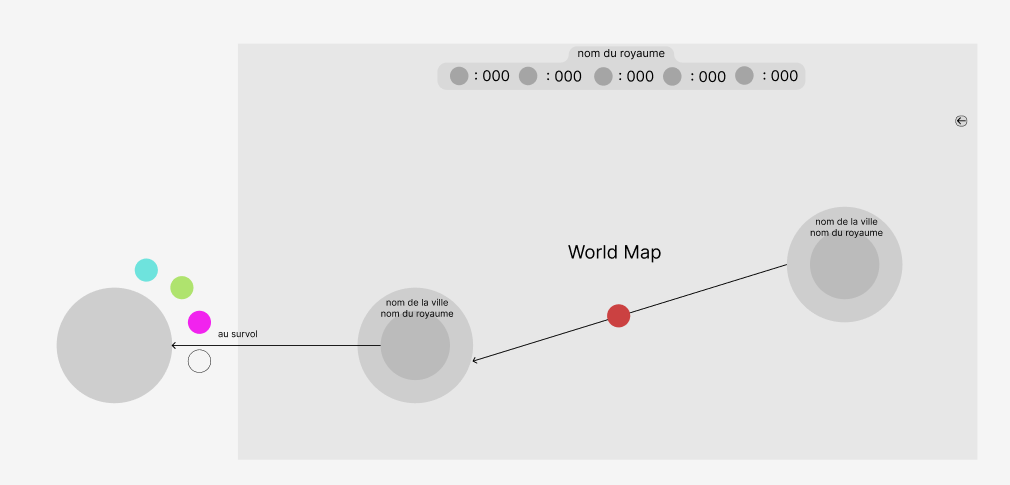
\includegraphics[width=0.7\linewidth]{images/figma_general.png}
    \caption{Schéma de l'interface en vue globale}
    \label{fig:figma-global}
\end{figure}

En cliquant sur une ville, le Seigneur accède à une interface spécifique lui permettant de consulter diverses informations telles que les bâtiments construits, ceux en cours de construction, et ceux dont il peut ordonner l’édification par les Péons.

\begin{figure}[!h]
    \centering
    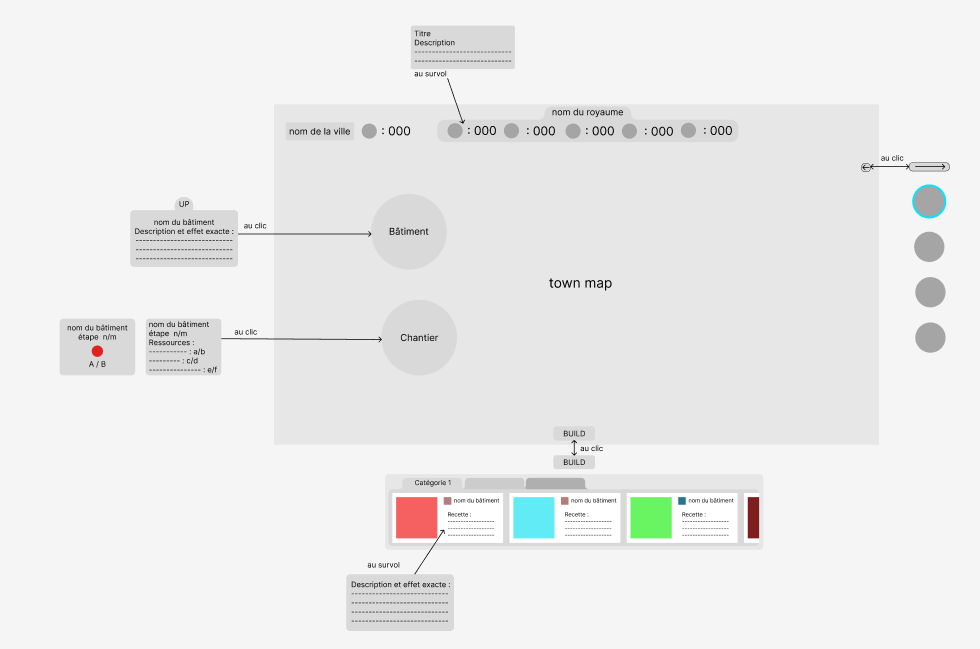
\includegraphics[width=0.7\linewidth]{images/figma_town.png}
    \caption{Schéma de l'interface de gestion de ville}
    \label{fig:figma-town}
\end{figure}

Un autre aspect important du rôle du Seigneur est la gestion diplomatique avec les autres royaumes. Il peut discuter en privé avec les autres Seigneurs, proposer des accords commerciaux, des alliances, ou encore déclarer des guerres.

\begin{figure}[!h]
    \centering
    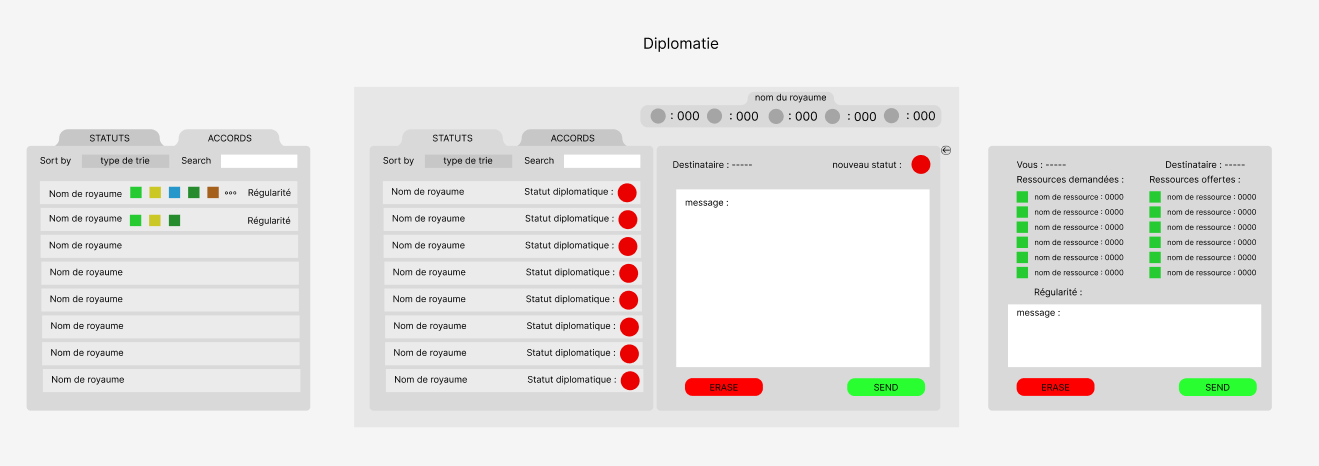
\includegraphics[width=0.7\linewidth]{images/figma_diplomatie.png}
    \caption{Schéma de l'interface diplomatique}
    \label{fig:figma-diplomacy}
\end{figure}

\newpage

\paragraph{Modélisation simplifiée des bâtiments}

Une contrainte importante réside dans la limitation des échanges d’informations entre le serveur et les clients, afin d’éviter une surcharge du réseau. Pour répondre à cette contrainte, nous avons choisi un système de représentation des bâtiments à la fois simple et efficace :

\begin{itemize}
  \item Chaque bâtiment possède un \textbf{type}, défini par son niveau, ainsi qu’un \textbf{état de santé} correspondant à son avancement dans le processus de construction.
  \item Lorsqu’un Seigneur place un nouveau bâtiment ou améliore un bâtiment existant, celui-ci commence avec \textbf{0 point de vie} et un \textbf{dictionnaire de ressources} listant les matériaux nécessaires pour l’étape de construction en cours.
  \item Les Péons apportent les ressources requises, complétant progressivement le dictionnaire.
  \item Une fois le dictionnaire complété, ils peuvent effectuer des \textit{mini-jeux de construction} pour augmenter les points de vie du bâtiment.
  \item Lorsqu’un seuil donné de points de vie est atteint, un nouveau dictionnaire est généré pour l’étape suivante, et le processus recommence.
\end{itemize}

Chaque bâtiment peut ainsi comporter plusieurs étapes de construction, chacune nécessitant un nombre variable de mini-jeux. Ce système permet de limiter les échanges réseau aux informations essentielles (état de santé et ressources), tandis que les détails des étapes sont stockés localement.

\newpage

\subsubsection{Le rôle du Péon}

Le gameplay du Péon est beaucoup plus simple. Son rôle consiste à exécuter les tâches élémentaires : il peut se déplacer librement sur la carte et interagir avec son environnement. Par exemple, interagir avec une ressource déclenche un mini-jeu qui détermine s’il parvient ou non à l’obtenir. Il peut ensuite transporter cette ressource, par exemple vers un chantier de construction.

Ce sont également les Péons qui construisent les bâtiments, via d'autres mini-jeux.

\paragraph{Mini-jeux}

Les Péons sont responsables de la collecte des ressources et de la construction des bâtiments. Pour rendre ces actions plus engageantes, nous avons décidé d’intégrer des mini-jeux simples à la place d’actions automatiques (comme cliquer sur un arbre pour obtenir du bois).

Ces mini-jeux prennent la forme de nouvelles scènes \texttt{Three.js} qui s’exécutent en dehors du système ECS principal(Qui sera détaillé dans la section concernant le moteur de jeu). Lorsqu’un joueur interagit avec une ressource ou un objet, une fenêtre de mini-jeu s’affiche au centre de son écran. Le type de mini-jeu dépend de l’action à effectuer, et plus le joueur réussit le mini-jeu, plus il obtient de ressources.

Par exemple, dans le mini-jeu de coupe du bois, le joueur doit effectuer des allers-retours avec sa souris, simulant une scie. Plus les mouvements sont efficaces, plus il récolte de bûches.